\section{Introduction}

\begin{figure}[!t]
\vskip -0.03in
  \centering
      {
        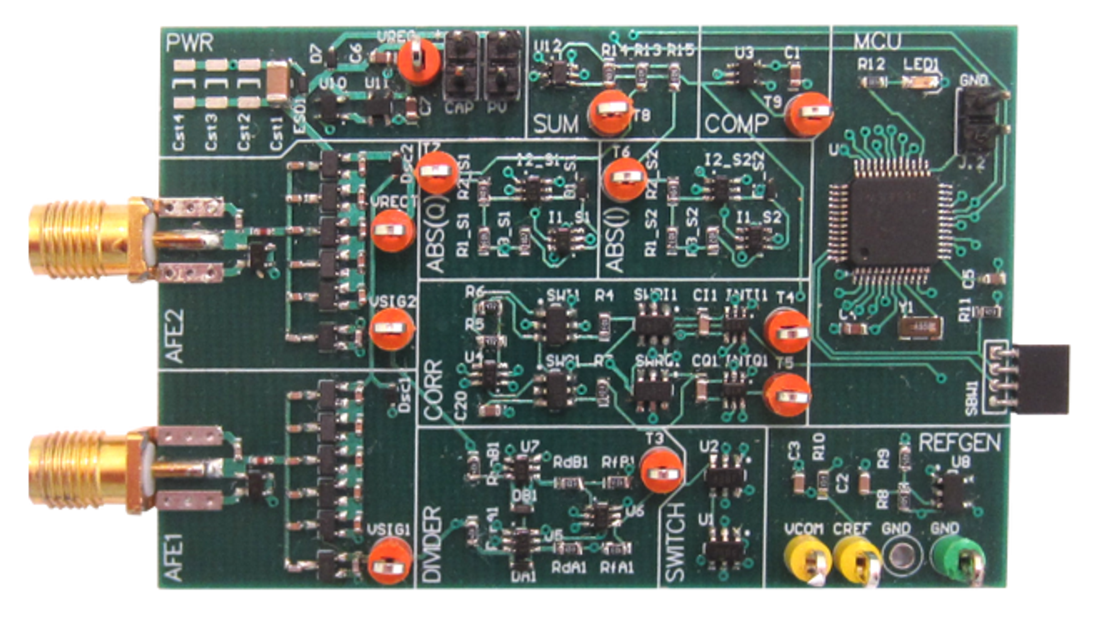
\epsfig{file=../figures/prototype-photo.eps, width=0.6\columnwidth}
      }
\caption{{\bf Our \vitag\ Prototype} \hl{integrates both mmm in a single design. It can operate using both RFID and TV transmissions}.}
\label{fig:tag}
\vskip -0.05in
\end{figure}

LEDs are prevalently deployed for illumination. This ubiquity opens a door for the LEDs to communicate with small computing devices through the vehicle of visible lights. The last few years have seen significant advances in VLC systems --- VLC systems today can achieve bit rates up to \hl{ss Mbps} from an LED transmitter to a receiver over a distance of \hl{ss}~\cite{flawedsys1,flawedsys2,flawedsys3,flawedsys4}. Researchers have also demonstrated the capability of providing location services using VLC~\cite{location1,location2}. These impressive capabilities are made possible by systems that encode and modulate the light emitted by the LED. However, all these systems, on one hand, either support only one-directional communication from the LED to the device where the device does not have the transmission capability, or entail the mobile device having additional LED~\cite{led2led1} or Bluetooth~\cite{ble1} facilities to transmit the uplink data; On the other hand, achieving such high data rate requires complicated modulation schemes and power-expensive analog-to-digital converters (ADCs) that consume power on the order of \hl{10mW}~\cite{flawedsys1}; this is orders of magnitude more power than is available on handhold devices that harvest power from ambient light sources.

In this paper, we ask if it is possible to achieve a bi-directional communication system on battery-free mobile devices only using the visible light as the carrier. Such a system would not only work at any location with LEDs at any time, but would also remedy the security flaws typically faced by existing RFID systems, where the uplink transmission tends to be exposed to a wide area of space, leaving chances for sniffers and attackers to temper the system. Thus, a positive answer would enable ubiquitous communication with access to existing network infrastructures at unprecedented spacial and temporal scales with user security preservation. 

Designing such a system, however, is challenging as (1) generating light waves and modulating them typically require much more power than can be harvested from ambient light sources by a small device (see~\ref{sec:app}), and moreover, (2) detecting signals sent by the device at the LED receiver against interferences is hard. In this paper, we introduce \vitag, a VLC system that provides duplex communication capabilities on battery-free devices only using visible light carriers. To address the challenge of detecting signals against interferences on the LED receiver, \vitag\ uses a novel algorithm specifically designed for the LCD-modulated signals. Instead of generating signals, \vitag\ addresses the power constraint challenge by backscattering the incoming light waves using retro-reflectors and modulating using Liquid-Crystal Displays (LCDs). This helps the backscattered signal focus at the receiver on the LED, and avoids generating signals on \vitag. In addition, \vitag\ recycles the LCD modulation energy with an energy reuse module, further optimizing the mobile device size to the size of a regular credit card. Finally, there are a set of other techniques behind the \vitag\ design that make it feasible in real-world illumination system deployment, which we will describe in later sections.

\textbf{\vitag.} To understand our \vitag\ design on battery-free ID card-sized tags, consider an LCD whose emitted light can be manipulated by an additional small circuit inside the light bulb. This circuit embeds information in the light and modulates it, while keeping the brightness of the light the same without any flickering. On the \vitag\ side, a light sensor captures the light signal that conveys information from the LED. To conserve energy, \vitag\ only uses analog components to demodulate the signal without an ADC. Upon detecting data, a low-power micro-controller on \vitag\ is waked up for uplink data transmission. It drives up the LCD to flicker, therefore sending data back to the LED by backscattering the light with a retro-reflector behind the LCD. This uplink data can be captured by a light sensor placed on the LED, along with interferences caused by downlink transmission, nearby human and object movements, household electricity fluctuations, and so on. A specifically designed receiver associated with the LED then performs the time recovery and demodulates the signal. To get a network of \vitag\/s and LEDs into play, we design a Media Access Control (MAC) protocol to mediate the communications in LEDs' illumination range. 

To show the feasibility of our ideas, we have built a hardware prototype, shown in Fig.~\ref{fig:tag}, that is approximately the size of a credit card. Our prototype includes multiple off-the-shelf LEDs emitting white lights, LED transmitters each stuffed inside an LED, LED receiver PCBs and \vitag\ PCBs. LEDs and \vitag\/s are equipped with a micro-controller, respectively. Our prototype also includes a solar cell of size \hl{ss $\times$ ss} on \vitag.

We evaluate our system in locations where illuminating LEDs are typically deployed, including office settings and evenings, as well as a dark chamber without other light sources as the baseline. We measure the longest communication range between the LED and \vitag, the area in which \vitag\ uplink transmission can be sniffed or tempered, and concurrent transmission capabilities. Our experiments show the following:

\begin{Itemize}
\item  Our \hl{ss $\times$ ss} \vitag\ prototype can achieve a bit rate of \hl{10kbps} on the downlink and \hl{1kbps} on the uplink at distances of up to \hl{2.2m} in dark chambers, \hl{2.0m} on sidewalks in the evening, and \hl{ss m} in offices, under the power budget of \hl{bb $\mu W$}.
\item \vitag's uplink transmission cannot be detected over the radius of \hl{m}, and malicious readers cannot detect uplink transmissions when tempering \hl{m} away from working \vitag\/s.
\item Via the MAC protocol described in Section~\ref{sec:mac}, \hl{blah}
\end{Itemize}

\vskip 0.05in\noindent{\bf Contributions:} We make the following contributions:
\begin{Itemize}
\item We present \vitag, the first visible light duplex communication system design that operates on battery-free devices while retaining a small size for them.
\item We develop a secure communication primitive applicable to RFID systems that acts against side sniffers and malicious transmitters.
\item Finally, we present designs and build a prototype which shows how all of the above, from \vitag, modified LEDs, through to the network stack, can be implemented on credit-card sized battery-free devices at a low cost.
\end{Itemize}


